% ICSA 2027 Research Papers Track — Double-Anonymous Submission
% Title: Verbatim Relay Fidelity of High-Entropy Credentials in LLM Tool Chains:
%        An Empirical Study and Reference Architecture
%
% Template: IEEEtran conference class (IEEE two-column format)
% Page limit: 10 pages main text (inclusive of figures, tables, appendices)
%             + 2 additional pages containing only references
%
% ANONYMISATION POLICY:
%   \anon{submitted text}{camera-ready text}
%   First argument is rendered in the submitted (anonymous) version.
%   Toggle to second argument for camera-ready by changing the macro definition.
%   Every usage is marked with a comment: % ANON: description
%
% EM-DASH PROHIBITION: Never use --- or \textemdash anywhere in this paper.
% Sync test: Overleaf ownership transferred to Jim Buckley 2026-09-02 - verifying git sync mechanics.
%   Use colons, semicolons, parentheses, or sentence restructuring instead.

\documentclass[conference]{IEEEtran}

% ─── Packages ────────────────────────────────────────────────────────────────
\usepackage[utf8]{inputenc}
\usepackage[T1]{fontenc}
\usepackage{microtype}   % character protrusion + font expansion; saves ~3-5 lines
\usepackage{enumitem}    % tight list spacing control
\usepackage{etoolbox}    % \patchcmd for post-init heading spacing tweaks
\usepackage{cite}
\usepackage{amsmath,amssymb}
\usepackage{graphicx}
\usepackage{xcolor}
\usepackage{booktabs}
\usepackage{multirow}
\usepackage{url}
\usepackage[hidelinks]{hyperref}
\usepackage{balance}  % balance final page columns
\usepackage{tabularx}

% ─── Float and caption spacing (space saving) ────────────────────────────────
\setlength{\textfloatsep}{6pt plus 2pt minus 4pt}
\setlength{\floatsep}{4pt plus 2pt minus 2pt}
\setlength{\dbltextfloatsep}{10pt plus 2pt minus 4pt}
\setlength{\dblfloatsep}{6pt plus 2pt minus 2pt}
\setlength{\abovecaptionskip}{2pt}
\setlength{\belowcaptionskip}{-4pt}

% ─── Section/subsection spacing — patched after IEEEtran's AtBeginDocument ──
% IEEEtran (conf) defines these at \begin{document}; patchcmd runs afterwards.
% Reduces after-skip (0.7ex→0.3ex) and before-skip (~0.5ex) across all headings.
\AtBeginDocument{%
  \patchcmd{\section}%
    {0.7ex plus 1ex minus 0ex}%
    {0.3ex plus 0.3ex minus 0ex}%
    {}{}%
  \patchcmd{\subsection}%
    {0.7ex plus .5ex minus 0ex}%
    {0.3ex plus 0.2ex minus 0ex}%
    {}{}%
}
\usepackage{array}
\usepackage{tikz}
\usetikzlibrary{arrows.meta, positioning, shapes.geometric, fit, backgrounds}

% ─── Anonymisation Toggle ────────────────────────────────────────────────────
% SUBMISSION VERSION (double-anonymous): renders first argument
% For camera-ready: change to \newcommand{\anon}[2]{#2}
\newcommand{\anon}[2]{#1}

% ─── Convenience Macros ──────────────────────────────────────────────────────
\newcommand{\RQ}[1]{\textbf{RQ#1}}
\newcommand{\Contrib}[1]{\textbf{C#1}}
\newcommand{\DFR}{\textrm{DFR}}
\newcommand{\ie}{\textit{i.e.}\xspace}
\newcommand{\eg}{\textit{e.g.}\xspace}
\newcommand{\cf}{\textit{cf.}\xspace}

% ─── Title ───────────────────────────────────────────────────────────────────
\title{Verbatim Relay Fidelity of High-Entropy Credentials\\in LLM Tool Chains: An Empirical Study\\and Reference Architecture}

% ─── Authors (anonymous for submission) ──────────────────────────────────────
% ANON: Replace with real author block for camera-ready
\author{
  \IEEEauthorblockN{Anonymous Authors}
  \IEEEauthorblockA{Paper ID: [To be assigned by EasyChair]\\
  Double-anonymous submission to ICSA 2027 Research Papers Track}
}

% ─── Document ────────────────────────────────────────────────────────────────
\begin{document}

\maketitle

% Abstract
% Section: Abstract
% Format: Verdecchia & Bogner (2025) structured abstract
%
% EM-DASH PROHIBITION: Do not use --- or \textemdash. Use colons or semicolons.

\begin{abstract}
Large Language Models (LLMs) increasingly orchestrate tool chains that invoke
external services. When such a chain carries an opaque cryptographic
credential, such as a JSON Web Token (JWT), the credential must remain
byte-for-byte unchanged: a one-character deviation can cause downstream
authentication to fail. We report a controlled experiment across
LLM-mediated Model Context Protocol (MCP) tool chains ($N\!=\!48{,}000$ \revjb{runs}
across 16 frontier LLMs), \revjb{a second condition using production-scale credentials}
($N\!=\!1{,}600$), and an industrial case
study. Across the controlled runs, the JWT Defect/Failure Rate (DFR) was
18.0\% (range 0.5--99.8\%; 12.5\% excluding the Mistral Large~3 outlier).
Failures increased with credential length, \revjb{and the corrupted bytes were
concentrated in the JWT payload segment}. In the \revjb{production-realistic condition},
an explicit relay instruction left
a residual DFR of 19.9\% ($+1.9$~pp, $p\!=\!0.16$), showing the mitigation
does not eliminate the failure. To address this integrity risk, we propose the
Credential Interception Vault, a reference architecture that separates
deterministic credential handling from probabilistic LLM orchestration, uses
credentials by reference, and is model-agnostic. By removing credentials from
the LLM inference path, the architecture eliminates direct byte relay by
construction; \revjb{we illustrate this approach in a production fintech deployment,
suggesting it largely removes downstream authentication failure}.
\end{abstract}


% Main sections
% Section 1: Introduction
% Source: context/Research_Questions_and_Contributions.md (GQM, 5 RQs, 7 contributions)
% Source: context/Paper_Layout_Plan.md §1 (structure notes)
% Source: context/Project Context_ LLM JWT Corruption in MCP Tool Chains.md §1-2 (problem statement)
%
% EM-DASH PROHIBITION: Do not use --- or \textemdash. Use colons or semicolons.

\section{Introduction}\label{sec:introduction}

The Model Context Protocol (MCP)~\cite{anthropic2024mcp} has rapidly become the
dominant interface for integrating Large Language Models (LLMs) into agentic
software systems~\cite{guo2025measurement,nsa2026mcp}. In a typical MCP deployment, an LLM orchestrator invokes
external tools by generating structured function calls, passing arguments from
one tool's output to the next. When those arguments include opaque, high-entropy
credentials such as JSON Web Tokens (JWTs)~\cite{rfc7519,rfc7518}, the LLM must relay them
\emph{verbatim}: a single altered character invalidates the RSA cryptographic
signature~\cite{rfc6750} and produces a hard authentication failure at the downstream API.

LLMs are probabilistic next-token predictors~\cite{vaswani2017attention} built on subword
tokenisation: Byte Pair Encoding (BPE~\cite{sennrich2016bpe}). They are not designed for byte-level verbatim
copying. When a high-entropy credential enters an LLM's context window, the
BPE tokeniser segments it into a non-uniform token sequence that does not
respect character boundaries. The LLM regenerates this sequence token by
token; we hypothesise this mechanism produces the character-level substitutions,
truncations, and semantic reinterpretations observed in our study. In privacy-preserving architectures where
authentication and signing occur locally and the resulting credential must be
relayed through an LLM orchestrator to a remote
API~\cite{anonymous2026issre}, any corruption causes a
non-recoverable authentication failure with no graceful fallback.

To our knowledge, no peer-reviewed study quantifies this failure rate, and no
published reference architecture addresses it. While adjacent work has studied LLM
hallucination~\cite{huang2025hallucination, ji2023hallucination}, secret
memorisation in code LLMs~\cite{nie2025decoding}, and MCP security risks through
static analysis~\cite{abadeh2026mcp}, the specific problem of \emph{runtime}
verbatim relay corruption of high-entropy credentials in live tool chains
has, to our knowledge, not been characterised in prior peer-reviewed work.

We advance the following research proposition:

\begin{quote}
\textit{For MCP deployments that relay cryptographic credentials through LLM
inference, our evidence strongly suggests that prompt-engineering mitigations
are insufficient to eliminate verbatim relay corruption under current frontier
models. A deterministic architectural bypass that removes the credential from
the LLM's inference path eliminates the failure mode in the systems studied,
independent of the model in use.}
\end{quote}

We structure the investigation around five research questions:

\begin{itemize}[itemsep=1pt,parsep=0pt,topsep=2pt]
  \item \RQ{1}: How prevalent is JWT corruption in LLM-mediated MCP relay, and
    how does it vary across the frontier model landscape?
  \item \RQ{2}: What is the structural and anatomical character of LLM JWT
    corruption events?
  \item \RQ{3}: To what extent can prompt-engineering mitigations reduce JWT
    corruption, and what prevents them from eliminating it?
  \item \RQ{4}: How does the Credential Interception Vault reference
    architecture structurally eliminate this failure mode?
  \item \RQ{5}: How is the Vault operationalised in production, and what
    evidence demonstrates its effectiveness?
\end{itemize}

This paper makes seven contributions.
The primary goal is to establish that the problem exists at meaningful scale
and that an architectural solution eliminates it; causal attribution of the
underlying mechanism is a declared direction for future work
(Section~\ref{sec:conclusion}).
\begin{enumerate}[itemsep=1pt,parsep=0pt,topsep=2pt]
    \item An empirical characterisation of JWT relay fidelity across 16
      frontier LLMs in 48{,}000 controlled L2 runs, producing a cross-model
      defect rate ranking (\Contrib{1}).
    \item A failure taxonomy distinguishing six outcome types with
      security severity ordering (\Contrib{2}).
    \item A corruption anatomy showing length-gated, payload-concentrated
      failure consistent with BPE tokenisation effects (\Contrib{3}).
    \item Empirical evidence that prompt engineering is insufficient to
      eliminate the corruption (19.9\% residual \DFR{} under production
      instruction conditions) (\Contrib{4}).
    \item The Credential Interception Vault, a facilitation-type reference
      architecture~\cite{angelov2012framework} that eliminates the failure by
      construction (\Contrib{5}).
    \item An industrial case study validating the architecture in a
      production blockchain trading system (\Contrib{6}).
    \item An open replication package (\Contrib{7}).
\end{enumerate}

Section~\ref{sec:related_work} surveys related work; Section~\ref{sec:study_design}
presents the design; Section~\ref{sec:results} reports \RQ{1}--\RQ{3}.
Sections~\ref{sec:reference_architecture}--\ref{sec:case_study} present the Vault RA and case study (\RQ{4}--\RQ{5}).
Sections~\ref{sec:discussion}--\ref{sec:conclusion} discuss, address threats, and conclude.

% Section 2: Related Work
% Source: context/Related Work Literature Review.md (all 5 areas)
% Source: context/ICSA_RA_Literature_Review.md §11 (reference quality, paper-section mapping)
% Source: context/ICSA_RA_Literature_Review.md §7.3 (Swiss Cheese differentiation)
% Source: context/ICSA_RA_Literature_Review.md §7.4 (ACE citation strategy)
% Source: context/ICSA_RA_Literature_Review.md §11.4 (Chen et al., Abadeh et al. differentiation)
%
% EM-DASH PROHIBITION: Do not use --- or \textemdash. Use colons or semicolons.

\section{Related Work}\label{sec:related_work}

\subsubsection*{LLM Output Fidelity}
LLM outputs are unreliable in ways that extend beyond factual
hallucination~\cite{huang2025hallucination, ji2023hallucination}. Nie et
al.~\cite{nie2025decoding} study how code LLMs handle secrets at the token
level, focusing on memorisation risk: the unintended reproduction of
training-data credentials. No prior work studies the complementary failure: the
\emph{corruption} of novel, unseen credentials when an LLM relays them at
inference time through a tool chain. This gap defines the empirical contribution
of the present study.

\subsubsection*{Tokenisation and String Integrity}
Byte Pair Encoding (BPE)~\cite{sennrich2016bpe} segments input into subword
tokens using merge rules from a training corpus. Applied to high-entropy strings
such as JWTs, BPE produces a non-uniform distribution that Chen et
al.~\cite{chen2026gibberish} term \emph{gibberish bias}: accidental
natural-language fragments (e.g., ``cut'' inside Base64url) merge into single
tokens while adjacent characters receive individual slots. Chen et al.\ measure
KL divergence of 2.668 between credential-string and normal-code token
distributions, and show the effect intensifies with vocabulary size (the current
scaling trajectory). We hypothesise this same distributional shift underlies
the relay fidelity failures we observe: rather than enabling memorised secret
reproduction, it impedes accurate relay of novel credential strings.
Chen et al.'s work concerns training-data secret \emph{leakage}, not
inference-time relay of novel credentials.

\subsubsection*{MCP and Agentic AI Security}
The Model Context Protocol~\cite{anthropic2024mcp} enables LLMs to invoke
external tools through structured function calls. Schick et
al.~\cite{schick2023toolformer} established that LLMs can learn tool use; He et
al.~\cite{he2025security} survey the resulting security and privacy risks
across the broader LLM agent landscape. Abadeh et al.~\cite{abadeh2026mcp}
provide the first peer-reviewed study of MCP-specific vulnerabilities, scanning
server configurations for privilege escalation and injection risks. Their
approach is complementary: static scanning examines infrastructure-level
configuration; our study addresses a runtime failure mode that arises during
live LLM inference and falls outside the scope of static analysis. Greshake et
al.~\cite{greshake2023prompt} and Liu et al.~\cite{liu2024prompt} study prompt
injection attacks on LLM-integrated applications; the Vault architecture we
propose incidentally mitigates indirect prompt injection targeting credentials,
as the credential never enters the LLM context.

\subsubsection*{Function-Call and Tool-Use Reliability}
Song et al.~\cite{song2025callnavi} find systematic argument misgeneration
in LLM function-calling across diverse API schemas; Yu
et al.~\cite{yu2026wildtoolbench} report compounding errors in multi-step
tool-use, with both studies tolerating near-miss outputs that constitute a hard
cryptographic failure in our setting. Haque et al.~\cite{haque2026verbatim}
study high-entropy string transcription failures in LLM code generation; that
work does not address credential relay.

\subsubsection*{Credential Relay in Distributed Systems}
The challenge of securely propagating bearer tokens across distributed
components is well-documented in microservice architectures. Yarygina and
Bagge~\cite{yarygina2018microservice} identify token propagation as a primary
security challenge in microservices. These patterns exist for deterministic
microservices, but they fail when a probabilistic LLM is introduced into the
relay chain: the LLM is not a transparent relay component but an active
transformer of its input. To our knowledge, no prior work addresses bearer
token integrity when the relay component is a stochastic language model.

\subsubsection*{Reference Architectures for LLM Agent Systems}
The Swiss Cheese Model for AI Safety~\cite{shamsujjoha2025swisscheese},
published at ICSA~2025, proposes a multi-layer guardrail reference architecture
for foundation model agents, inspired by Reason's accident causation model~\cite{reason1990human}. While
conceptually adjacent, it addresses general agent failure modes (hallucination,
misalignment, prompt injection) through stacked defensive layers. The failure
mode we study is distinct: verbatim credential relay corruption produces
well-formed but cryptographically invalid output that passes format validation at
every Swiss Cheese layer. Our architectural response is also distinct: rather
than adding layers around LLM inference, the Credential Interception Vault
removes the credential from the inference path entirely. The two architectures
are complementary. Li et al.'s ACE architecture~\cite{li2026ace}, published at
NDSS~2026, isolates LLM plan generation from deterministic execution to prevent
prompt injection. We apply the same separation principle to a different failure
mode: verbatim string relay fidelity. In both cases, deterministic correctness
guarantees cannot be provided by a probabilistic component, regardless of the
operation's apparent simplicity.

Grammar-constrained decoding~\cite{geng2023grammar} cannot guarantee byte-level
fidelity of opaque strings: BPE tokenisation fragments the credential before
generation begins, and no grammar can reconstruct a specific byte sequence
already split across merge boundaries. OAuth~2.0 Token Exchange
(RFC~8693~\cite{rfc8693}) assumes a deterministic relay agent; the stochastic
byte-level transformation we measure is outside its threat model.

The RA canon provides the classification framework for our contribution.
Following Angelov et al.~\cite{angelov2012framework}, we classify the Vault as
a Type~2 facilitation-type RA: designed by researchers to guide practitioners,
with voluntary adoption. Galster and Avgeriou~\cite{galster2011empirically}
propose a six-step methodology for empirically-grounded RAs; our study
satisfies all six steps (Section~\ref{sec:ra_type}).



% Section 3: Study Design
% Source: context/Empirical Evaluation Design (full)
% Source: context/Statistical Analysis Plan (full)
% Source: context/Paper_Layout_Plan.md §3
%
% EM-DASH PROHIBITION: Do not use --- or \textemdash. Use colons or semicolons.

\section{Study Design}\label{sec:study_design}

The goal is to establish that JWT relay corruption is systematic
(not model-specific), to quantify the limits of prompt-based mitigation, and to
validate an architectural solution in production. A controlled
experiment~\cite{shull2008guide} measures prevalence and effect sizes; an industrial case
study~\cite{runeson2009case} provides contextual validation. The ecological
validity arm bridges the two using production artifacts within the controlled
framework.

The study follows Verdecchia and Bogner~\cite{verdecchia2025notes} and
Kitchenham et al.~\cite{kitchenham2001guidelines}.
Sections~\ref{sec:objects}--\ref{sec:analysis_plan} describe the experiment;
Section~\ref{sec:case_study} presents the case study design and findings
together~\cite{runeson2009case}. Figure~\ref{fig:methodology} summarises the
overall process flow, from JWT generation through the main experiment and
ecological validity arms to statistical analysis; the industrial case study
(dashed, external) supplies the production tool schema that grounds the
ecological validity arm.

\begin{figure*}[t]
  \centering
  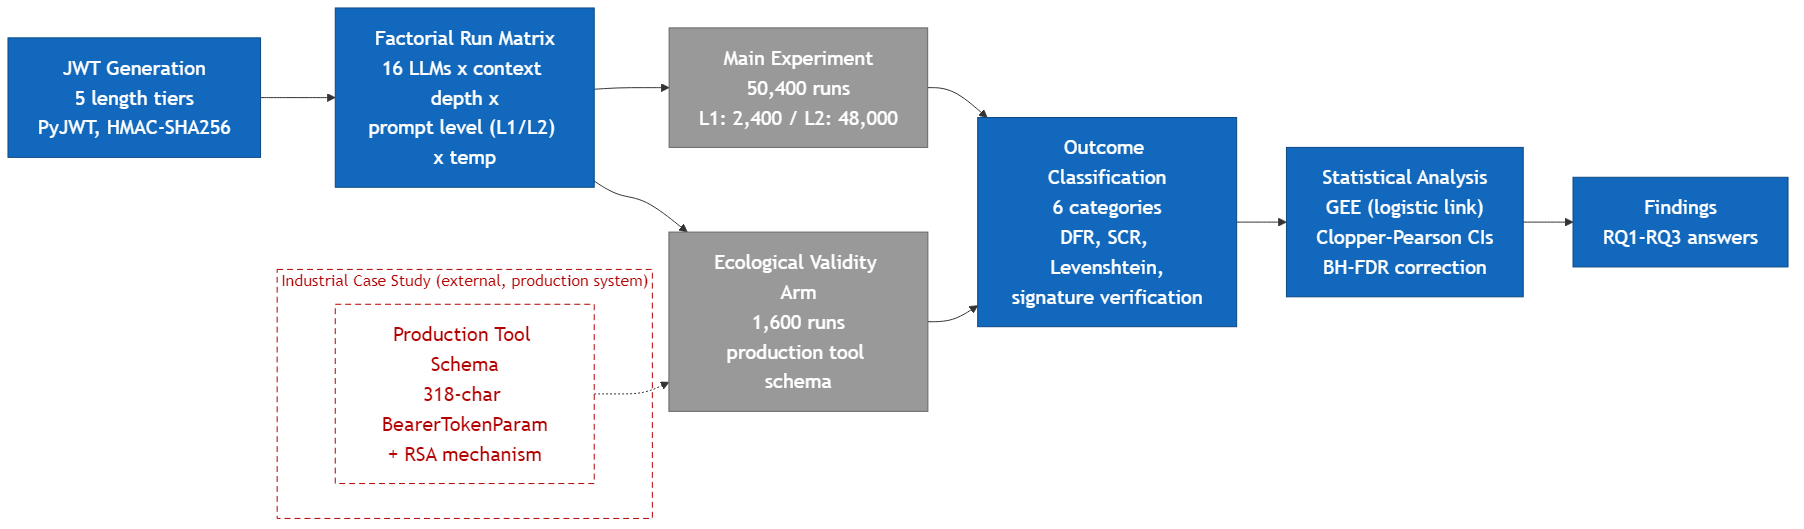
\includegraphics[width=0.75\textwidth]{figures/fig00_methodology_flow.png}
  \vspace{-4pt}\caption{Overall methodology process flow. Blue stages are
  common pipeline steps; grey stages are the two experimental arms. The
  dashed box denotes the industrial case study (Section~\ref{sec:case_study}),
  an external, production system that supplies the tool schema grounding the
  ecological validity arm.}
  \label{fig:methodology}
\end{figure*}

\subsection{Experimental Objects}\label{sec:objects}

The experimental objects are synthetic JWTs generated per-run using
\texttt{PyJWT} with a fresh HMAC-SHA256 secret and a randomised payload
containing a UUID, Unix timestamp, user identifier, and nested JSON claims.
Two design decisions motivate synthetic rather than real tokens. First, real
JWTs from known systems risk appearing in LLM training data, introducing a
contamination threat that synthetic tokens eliminate. Second, synthetic tokens
allow cryptographic signature verification as an independent ground-truth check
on corruption measurement.

JWTs are generated at five length tiers (Table~\ref{tab:jwt_tiers}) to test
the relationship between credential length and defect rate.

\begin{table}[t]
\centering
\small
\vspace{-4pt}\caption{JWT length tiers.}
\label{tab:jwt_tiers}
\begin{tabular}{@{}llp{3.8cm}@{}}
\toprule
\textbf{Tier} & \textbf{Target} & \textbf{Rationale} \\
\midrule
Short        & $\sim$200 chars & Minimal realistic JWT  \\
Medium low   & $\sim$300 chars & Below-typical; tests early-onset corruption \\
Medium       & $\sim$500 chars & Typical production JWT \\
Long         & $\sim$900 chars & Complex claims (e.g., role arrays) \\
Very long    & $\sim$1{,}400 chars & Upper extreme; production RS256 token ($\sim$1{,}080 chars) falls in this tier \\
\bottomrule
\end{tabular}
\end{table}

\subsection{Experimental Subjects}\label{sec:subjects}

Sixteen LLMs were selected across eight tiers (Table~\ref{tab:models}) to
provide broad coverage of the 2026 frontier landscape. The selection follows
current guidelines for empirical SE studies involving
LLMs~\cite{verdecchia2025notes}, requiring commercial frontier models,
open-source baselines, and longitudinal pairs (two Claude Sonnet generations,
two Google Gemini generations) to test whether model-generation advancement
reduces corruption. Chinese and European frontier models are included because
different training corpora may produce tokenisers with different Base64url
segmentation behaviour.

\begin{table*}[t]
\centering
\small
\vspace{-4pt}\caption{Model taxonomy. All models were API-version pinned at the start of
data collection. Tier codes: WF=Western Frontier, CE=Cost-Efficient,
R=Reasoning, CF=Chinese Frontier, EF=European Frontier, LB=Legacy Baseline,
SL=Sonnet Longitudinal, GL=Google Longitudinal, LO=Local/Open-weight.}
\label{tab:models}
\setlength{\tabcolsep}{6pt}
\begin{tabular}{@{}lll@{\qquad\qquad}lll@{}}
\toprule
\textbf{Model} & \textbf{Tier} & \textbf{Provider} &
\textbf{Model} & \textbf{Tier} & \textbf{Provider} \\
\midrule
Claude Sonnet 5       & WF & Anthropic  & Mistral Large 3       & EF & Mistral \\
Gemini 3.5 Flash      & WF & Google     & Mistral Small 4       & EF & Mistral \\
GPT-5.4-mini          & CE & OpenAI     & GPT-4o (pinned)       & LB & OpenAI \\
Claude Haiku 4.5      & CE & Anthropic  & Claude Sonnet 4.5     & SL & Anthropic \\
Gemini 3.1 Flash-Lite & CE & Google     & Claude Sonnet 4.6     & SL & Anthropic \\
o4-mini               & R  & OpenAI     & Gemini 3 Flash        & GL & Google \\
DeepSeek V3           & CF & DeepSeek   & Gemini 2.5 Flash      & GL & Google \\
GLM-4 Flash           & CF & Zhipu AI   & Gemma 4 E4B           & LO & Ollama \\
\bottomrule
\end{tabular}
\end{table*}

\subsection{Variables}\label{sec:variables}

\textbf{Independent variables.}
The experiment uses a mixed factorial design:
(1)~JWT length tier (5~levels: short, medium-low, medium, long, very-long);
(2)~context depth (3~levels: shallow~$\sim$100 tokens, medium~$\sim$1{,}500,
    deep~$\sim$3{,}000 tokens);
(3)~prompt ecological level (2~levels: L1, L2);
and (4)~temperature ($T\!=\!0.0$ and $T\!=\!0.7$).
L2 was run at all factor combinations (100 iterations per cell); L1
at a single temperature and medium context depth to bound cost.
The 15 API-hosted models each completed 3{,}000 L2 target runs; Gemma~4~E4B
(Ollama local) completed 3{,}000 L2 runs, yielding 48{,}000 total L2 runs
(100\% of the 48{,}000 API-model target).
L1 contributed 2{,}400 runs (16 models $\times$ 150 iterations across five
JWT-length tiers, single temperature, medium context depth), bringing the
combined main-arm total to 50{,}400. With the eco arm ($N\!=\!1{,}600$;
Section~\ref{sec:eco_arm}), the overall study comprises 52{,}000 completed
runs.

\textbf{Dependent variables.}
The primary outcome is the \emph{Defect/Failure Rate} (\DFR{}): a binary
indicator coded 1 if the output does not byte-for-byte match the input JWT. For
corrupted runs, we compute the Levenshtein distance to measure severity and the
Segment Corruption Rate (SCR) per JWT segment (header, payload, signature).
Cryptographic signature verification provides an independent ground-truth check.

Outcomes are classified into six mutually exclusive categories
(Table~\ref{tab:taxonomy}, Section~\ref{sec:rq2}). \textit{Semantic
substitution} is assigned when the output contains no dot-separated
Base64url triplet but is non-empty (UUID extraction, JSON expansion,
claim-value repetition). The replication package contains verbatim
prompt templates, API model identifiers, SDK versions, tool schemas, request/response extraction, and error-handling
logic.

\subsection{Ecological Validity Arm}\label{sec:eco_arm}

To test whether prompt-engineering mitigations can close the gap under
production conditions, we conduct an ecological validity arm ($N\!=\!1{,}600$;
16 models $\times$ 100 iterations) using the exact JWT schema and the
verbatim 318-character \texttt{BearerTokenParam} tool instruction from the
production codebase (Section~\ref{sec:case_study}), which names the RSA
mechanism and warns that any single changed character produces a 403~error.
A \texttt{RESEARCH\_RAW\_MODE} flag bypasses production mitigations.
The pre-specified test is Spearman's $\rho$ between eco arm and main
experiment model rankings.

\subsection{Analysis Plan}\label{sec:analysis_plan}

Between-model inference uses Generalised Estimating Equations (GEE) with
logistic link, binomial family, and exchangeable working correlation, clustered
at the (model, cell) level. GEE estimates population-average effects and is
robust to correlation misspecification via the sandwich variance
estimator~\cite{kitchenham2001guidelines}. Per-model \DFR{} estimates use
Clopper-Pearson exact binomial 95\% confidence intervals. Pairwise comparisons
use Benjamini-Hochberg FDR correction at $\alpha\!=\!0.05$. The eco arm uses
Spearman's $\rho$ for rank correlation and Mann-Whitney~$U$ for the vocabulary
effect test.

% Section 4: Results
% Source: context/Discussion_and_Conclusions.md §D2-D4, §D12
% Source: context/Paper_Layout_Plan.md §4
%
% EM-DASH PROHIBITION: Do not use --- or \textemdash. Use colons or semicolons.

\section{Empirical Study Results}\label{sec:results}

A total of 50{,}400 runs completed (48{,}000 at L2, the primary analysis
condition; 2{,}400 at L1). We report
results organised by research question.

\subsection{RQ1: Prevalence and Cross-Model Variation}\label{sec:rq1}

The pre-declared primary aggregate is pooled \DFR{} across all 16~models
at L2 (48{,}000 runs); the 15-model figure excluding the Mistral~Large~3
outlier is a pre-specified sensitivity check.

The overall JWT Defect/Failure Rate across 16 models under L2 conditions was
\textbf{18.0\%} (95\% CI: [17.6\%, 18.3\%]). Approximately one in six
authenticated tool-chain invocations produced a cryptographically invalid JWT.

Per-model \DFR{} ranged from \textbf{0.5\% to 99.8\%}
(Table~\ref{tab:failure_matrix}, Figure~\ref{fig:dfr_model}).
No model achieved zero \DFR{}.

\textbf{Outlier analysis: Mistral Large~3.}
Mistral Large~3 (99.8\% \DFR{}, 3{,}000 L2 runs) is qualitatively distinct.
Manual inspection of 50~outputs confirms explanation-mode semantic substitution
as the dominant failure (99.0\%): the model returns a description rather than
the credential. Two causes are consistent:
(i)~a \emph{tokenisation artifact} (aggressive BPE fragmentation favouring
paraphrase), or (ii)~a \emph{model-configuration artifact} (the pinned
version's instruction-following profile prioritising explanation).
The implication is that some models may be inherently unsuitable for direct
credential relay, strengthening the case for an architectural bypass. Excluding this outlier, pooled \DFR{} is
\textbf{12.5\%} (95\% CI: [12.2\%, 12.8\%], $N\!=\!45{,}000$, 15~models),
confirming that the headline finding is not driven by a single outlier.
BH-corrected pairwise Fisher's exact tests across all
$\binom{16}{2}\!=\!120$ model pairs found 110 of 120 pairs (92\%) significantly
different at $\alpha\!=\!0.05$, confirming near-universal heterogeneity.

\begin{figure}[t]
  \centering
  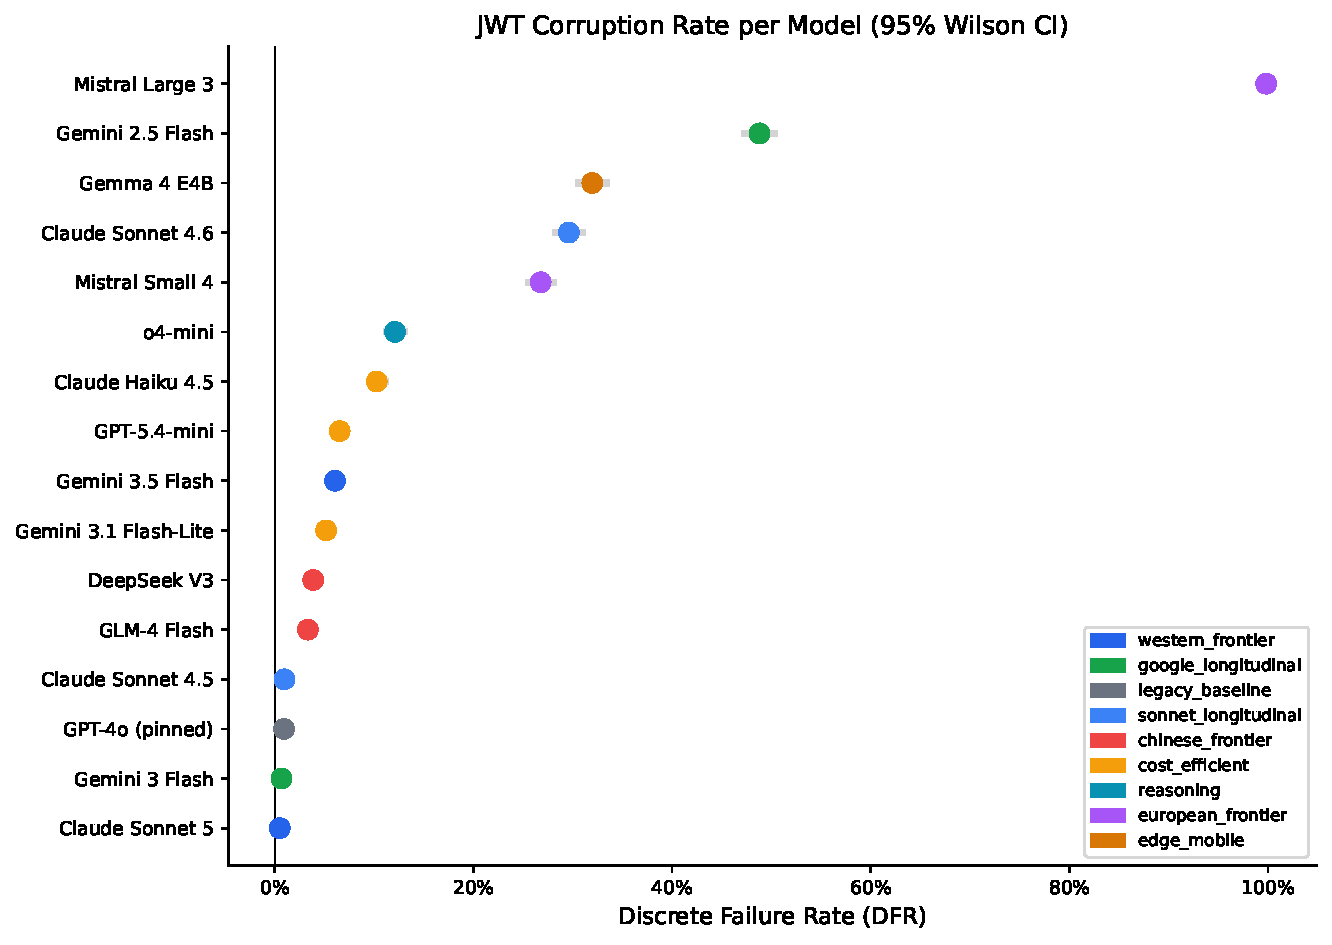
\includegraphics[width=0.82\columnwidth]{figures/fig01_dfr_by_model.pdf}
  \vspace{-4pt}\caption{Per-model JWT Defect/Failure Rate with Clopper-Pearson 95\%
  confidence intervals, sorted ascending and grouped by tier.}
  \label{fig:dfr_model}
\end{figure}

% Table 4: Per-model failure-type breakdown matrix
\begin{table*}[t]
\centering
\footnotesize
\vspace{-4pt}\caption{Per-model failure-type breakdown. Values are percentages of total L2 runs per model. \DFR{} = $1 -$ Exact Match \%.
Clopper-Pearson 95\% CIs reported for \DFR{} only.}
\label{tab:failure_matrix}
\begin{tabular}{@{}llrrrrrr@{}}
\toprule
\textbf{Model} & \textbf{Tier} & \textbf{Exact \%} & \textbf{Corrupt \%} & \textbf{Sem.Sub \%} & \textbf{Abst \%} & \textbf{DFR \%} & \textbf{95\% CI} \\
\midrule
% Data extracted from reports/parquet/main_l2.parquet (N=48,000 L2 runs)
% Sorted by DFR descending. Corrupt\% merges corrupted + truncated categories.
% Note: Refusal rate was 0.0\% for all 16 models and is omitted from this table.
Mistral Large 3          & EF & 0.2  & 0.0  & 99.0 & 0.8 & 99.8 & [99.6, 99.9] \\
Gemini 2.5 Flash         & GL & 51.2 & 48.7 & 0.0  & 0.1 & 48.8 & [47.0, 50.6] \\
Claude Sonnet 4.6        & SL & 70.4 & 0.6  & 28.0 & 1.0 & 29.6 & [28.0, 31.3] \\
Gemma 4 E4B              & LO & 68.0 & 28.9 & 1.4  & 1.7 & 32.0 & [30.3, 33.7] \\
Mistral Small 4          & EF & 73.2 & 22.4 & 4.2  & 0.2 & 26.8 & [25.2, 28.4] \\
\midrule
o4-mini                  & R  & 87.9 & 5.4  & 0.0  & 6.7 & 12.1 & [11.0, 13.3] \\
Claude Haiku 4.5         & CE & 89.7 & 10.0 & 0.3  & 0.0 & 10.3 & [9.2, 11.4] \\
GPT-5.4-mini             & CE & 93.5 & 6.5  & 0.0  & 0.0 & 6.5  & [5.7, 7.5] \\
Gemini 3.5 Flash         & WF & 93.9 & 5.2  & 0.0  & 0.9 & 6.1  & [5.2, 7.0] \\
Gemini 3.1 Flash-Lite    & CE & 94.8 & 0.4  & 4.7  & 0.0 & 5.2  & [4.4, 6.0] \\
\midrule
DeepSeek V3              & CF & 96.1 & 3.8  & 0.1  & 0.0 & 3.9  & [3.2, 4.6] \\
GLM-4 Flash              & CF & 96.7 & 1.8  & 0.0  & 1.6 & 3.3  & [2.7, 4.0] \\
Claude Sonnet 5          & WF & 99.5 & 0.5  & 0.0  & 0.0 & 0.5  & [0.3, 0.8] \\
Claude Sonnet 4.5        & SL & 99.0 & 1.0  & 0.0  & 0.0 & 1.0  & [0.6, 1.4] \\
GPT-4o (pin.)            & LB & 99.1 & 0.5  & 0.5  & 0.0 & 0.9  & [0.6, 1.3] \\
Gemini 3 Flash           & GL & 99.3 & 0.7  & 0.0  & 0.0 & 0.7  & [0.4, 1.0] \\
\midrule
\textbf{All models (N=48,000)} & & 82.0 & 8.5 & 8.6 & 0.8 & \textbf{18.0} & [17.6, 18.3] \\
\bottomrule
\end{tabular}
\end{table*}

No model exhibited safety-based refusal (0.0\%; see taxonomy,
Table~\ref{tab:taxonomy}). Cost-efficient models do not uniformly exhibit
higher \DFR{} than frontier models. The reasoning-tier model (o4-mini) shows a distinctive profile:
chain-of-thought inference fragments credentials through an additional
generation layer. Chinese frontier models show \DFR{} consistent with
different BPE vocabularies from Chinese-dominant corpora.

\subsection{RQ2: Structural Anatomy of Corruption}\label{sec:rq2}

\textbf{Length-gating.}
\DFR{} increases monotonically across tiers (Figure~\ref{fig:length_trend}):
short~12.6\%, medium-low~12.6\%, medium~13.6\%, long~22.2\%, very-long~28.7\%
(Spearman $\rho\!=\!0.900$, $p\!=\!0.037$). A Mantel-Haenszel test
(high tiers: long\,+\,very-long vs.\ low tiers: short\,+\,medium-low;
16~model strata) confirms a significant length effect:
OR~=~4.785 (95\% CI: [1.14, 20.0], $p\!<\!0.001$).
This result is identical when Mistral~Large~3 is excluded
(OR~=~4.785, 15~strata, $p\!<\!0.001$), confirming the length effect
is not an artefact of that single outlier.
Context depth DFR is monotonically increasing across three levels
($\rho\!=\!1.000$; $n\!=\!3$ precludes a meaningful permutation $p$-value);
A within-model GEE (groups\ =\ model, controlling for JWT length tier)
yields OR~=~1.093 (95\% CI: [0.84,~1.42], $p\!=\!0.51$), indicating no
statistically significant independent context effect once model identity
and token-length are held constant.

\begin{figure*}[t]
  \centering
  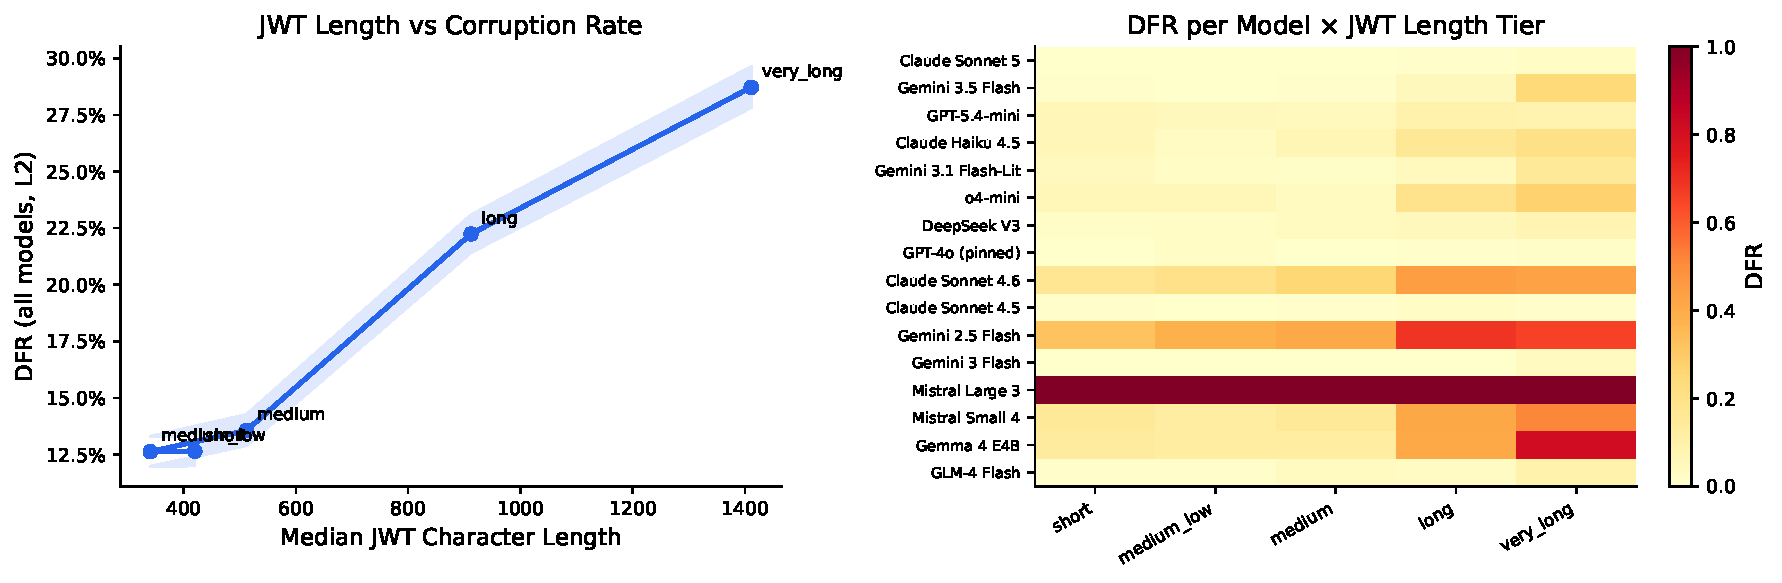
\includegraphics[width=0.82\textwidth]{figures/fig02_length_trend.pdf}
  \vspace{-4pt}\caption{\DFR{} by JWT length tier and context depth (left) and per-model
  \DFR{} heatmap across length tiers (right). The onset of non-trivial
  corruption occurs at $\sim$200 characters.}
  \label{fig:length_trend}
\end{figure*}

\textbf{Segment analysis.}
Segment Corruption Rate (SCR) analysis reveals that payload corruption dominates:
among character-level failures, 92.8\% involve payload mismatch, followed by
signature (11.3\%) and header (0.4\%). For the synthetic HS256 tokens used, the
payload is the longest Base64url segment; this segment-level length-gating mirrors
the JWT-level finding, consistent with BPE boundary exposure scaling with segment
length.
Among corrupted runs, 41.0\% show single-character substitution
(Levenshtein $L\!=\!1$) and 35.1\% show $L>5$ (mean $L\!=\!59.5$, pulled
upward by near-total rewrites), indicating a bimodal severity distribution.
DFR at fully deterministic sampling ($T\!=\!0.0$) was 17.3\%, only 1.3~pp
below $T\!=\!0.7$ (18.6\%), confirming the dominant failure mode is
deterministic, not sampling-noise-driven.

\textbf{Failure taxonomy.}
Table~\ref{tab:taxonomy} presents the six-outcome taxonomy (\Contrib{2}).
Character-level corruption (Levenshtein $\geq 1$, modal distance $L\!=\!1$) is
the dominant failure mode. Truncation (credential cut short) is a structurally
distinct sub-mode observed in 0.4\% of runs and reported merged with
\texttt{corrupted} in Table~\ref{tab:failure_matrix}. Semantic substitution,
where the LLM decodes the JWT payload and returns a plausible but
cryptographically invalid value, is rare but architecturally critical: it is
undetectable by any validation mechanism that does not hold a reference copy of
the original token.

\begin{table}[t]
\centering
\footnotesize
\vspace{-4pt}\caption{Six-outcome taxonomy of JWT relay results (\Contrib{2}). The
architectural implication column motivates the design decisions in
Section~\ref{sec:reference_architecture}. \texttt{refusal} had 0.0\%
observation rate in this study but is architecturally relevant
(Section~\ref{sec:ra_motivation}).}
\label{tab:taxonomy}
\begin{tabular}{@{}lp{4.5cm}@{}}
\toprule
\textbf{Outcome} & \textbf{Architectural Implication} \\
\midrule
\texttt{exact\_match}  & No intervention required \\
\texttt{corrupted}     & Interceptor must hold reference copy \\
\texttt{truncated}     & Credential shortened; same cryptographic impact as corrupted \\
\texttt{sem\_sub}      & Levenshtein detection insufficient; credential must not pass through LLM \\
\texttt{abstention}    & LLM cannot be relied upon for credential forwarding \\
\texttt{refusal}       & Out-of-band credential passing is the only solution \\
\bottomrule
\end{tabular}
\end{table}

\subsection{RQ3: Prompt Engineering as Insufficient Mitigation}\label{sec:rq3}

The L1$\rightarrow$L2 prompt transition produces a marginal, non-significant
change in overall \DFR{} ($+1.1$~pp, $p\!=\!0.18$), confirming that
increased instruction detail did not eliminate the observed corruption.

The ecological validity arm ($N\!=\!1{,}600$) provides the key measurement
under production conditions. Using the production \texttt{BearerTokenParam} instruction
(318~characters, explicitly naming the RSA signature consequence), the \DFR{}
was \textbf{19.9\%}. The difference from the main study at the same length tier
was $+1.9$~percentage points ($p\!=\!0.16$, Wilcoxon; not
significant). Spearman's rank correlation between eco arm and main experiment
model rankings was $\rho\!=\!0.740$ ($p\!=\!0.001$), confirming that model
rankings transfer to production conditions.

The most explicit instruction achievable within the MCP tool schema design space
produces a result statistically indistinguishable from neutral vocabulary.
Corruption persists regardless of prompt specificity; BPE tokenisation boundaries
appear to operate below the level of instruction-following behaviour and were not
overcome by any prompt tested in this study. We note that non-significance alone
does not constitute formal equivalence: establishing a true prompt ceiling would
require pre-specified equivalence margins and a TOST procedure, which is
identified as future work (Section~\ref{sec:conclusion}).

% Section 5: Reference Architecture
% Source: context/ICSA_RA_Literature_Review.md §1-8, §12
% Source: context/Paper_Layout_Plan.md §5
%
% EM-DASH PROHIBITION: Do not use --- or \textemdash. Use colons or semicolons.

\section{Reference Architecture}\label{sec:reference_architecture}

\subsection{From Taxonomy to Architectural Requirements}\label{sec:ra_motivation}

The six-outcome taxonomy (Table~\ref{tab:taxonomy}) is not merely a
measurement scheme; each outcome implies a specific architectural requirement.
Character-level corruption (\texttt{corrupted}) requires a reference copy for
verification. Semantic substitution (\texttt{sem\_sub}), where the LLM decodes
the JWT payload and returns a plausible but cryptographically invalid value, is
undetectable by format validation, length checking, or bounded Levenshtein
comparison: the only complete mitigation is to prevent the LLM from processing
the credential at all. Model refusal (\texttt{refusal}) and abstention
(\texttt{abstention}) mean the architecture cannot depend on the LLM forwarding
the credential. The only mechanism that covers all five outcome categories is
bypassing the LLM for credential relay entirely.

\subsection{RA Type and Design Principles}\label{sec:ra_type}

Following Angelov et al.~\cite{angelov2012framework}, we classify the
Credential Interception Vault as a \emph{Type~2 facilitation-type} reference
architecture: designed to guide practitioners building privacy-preserving MCP
agent systems, with voluntary adoption. The architecture is empirically grounded following Galster and
Avgeriou's~\cite{galster2011empirically} six steps: problem identification
(Section~\ref{sec:introduction}); evidence collection ($N\!=\!50{,}400$ runs);
requirement derivation (six-outcome taxonomy, above); architecture proposal
(this section); validation (eco arm and production, Section~\ref{sec:case_study});
and documentation (this paper and replication package).

The architecture rests on three design principles:

\textbf{P1: Deterministic Shell, Probabilistic Core.}
The LLM (the probabilistic core) reasons about intent and selects tool
invocations. The Vault (the deterministic shell) executes credential injection
with correctness guarantees independent of the LLM's inference quality. This
embodies what Amodei et al.~\cite{amodei2016concrete} identify as a necessary
property of safe AI systems: deterministic oversight of probabilistic
components. The Vault instantiates the Interceptor pattern from
POSA~\cite{buschmann2007posa4} and is consistent with the decide/execute
separation in Li et al.'s ACE architecture~\cite{li2026ace}.

\textbf{P2: Credentials by Reference, Not by Value.}
The LLM never receives the raw credential. It receives an opaque reference
handle that carries no information about the credential's content. The Vault
resolves the handle to the cached credential at injection time.

\textbf{P3: Model-Agnostic Guarantee.}
The correctness guarantee holds regardless of which LLM is in use. The Vault
operates at the MCP middleware layer, below the inference layer; swapping the
underlying model requires no changes to the Vault.

\subsection{Architecture Overview}\label{sec:c4}

Figure~\ref{fig:c4} presents the C4 container-level
view~\cite{brown2018c4}.\footnote{The label \emph{C4} here denotes the
four-level container-diagram notation of Brown~\cite{brown2018c4}; it is
unrelated to the contribution identifier \Contrib{4} used in
Sections~\ref{sec:introduction} and~\ref{sec:conclusion}.}
The system boundary contains five
containers. The \emph{Credential Interception Vault} (centre, bold) is the
architectural invariant: its intercept-cache-inject behaviour is fixed across
all instantiations. All other containers are variability points
(\texttt{[VP]}) that differ across deployments. The trust boundary (dashed)
encloses the Vault and, in privacy-critical deployments, the
Credential-Bearing Tool; credentials never cross this boundary to
untrusted environments.

\begin{figure*}[t]
  \centering
  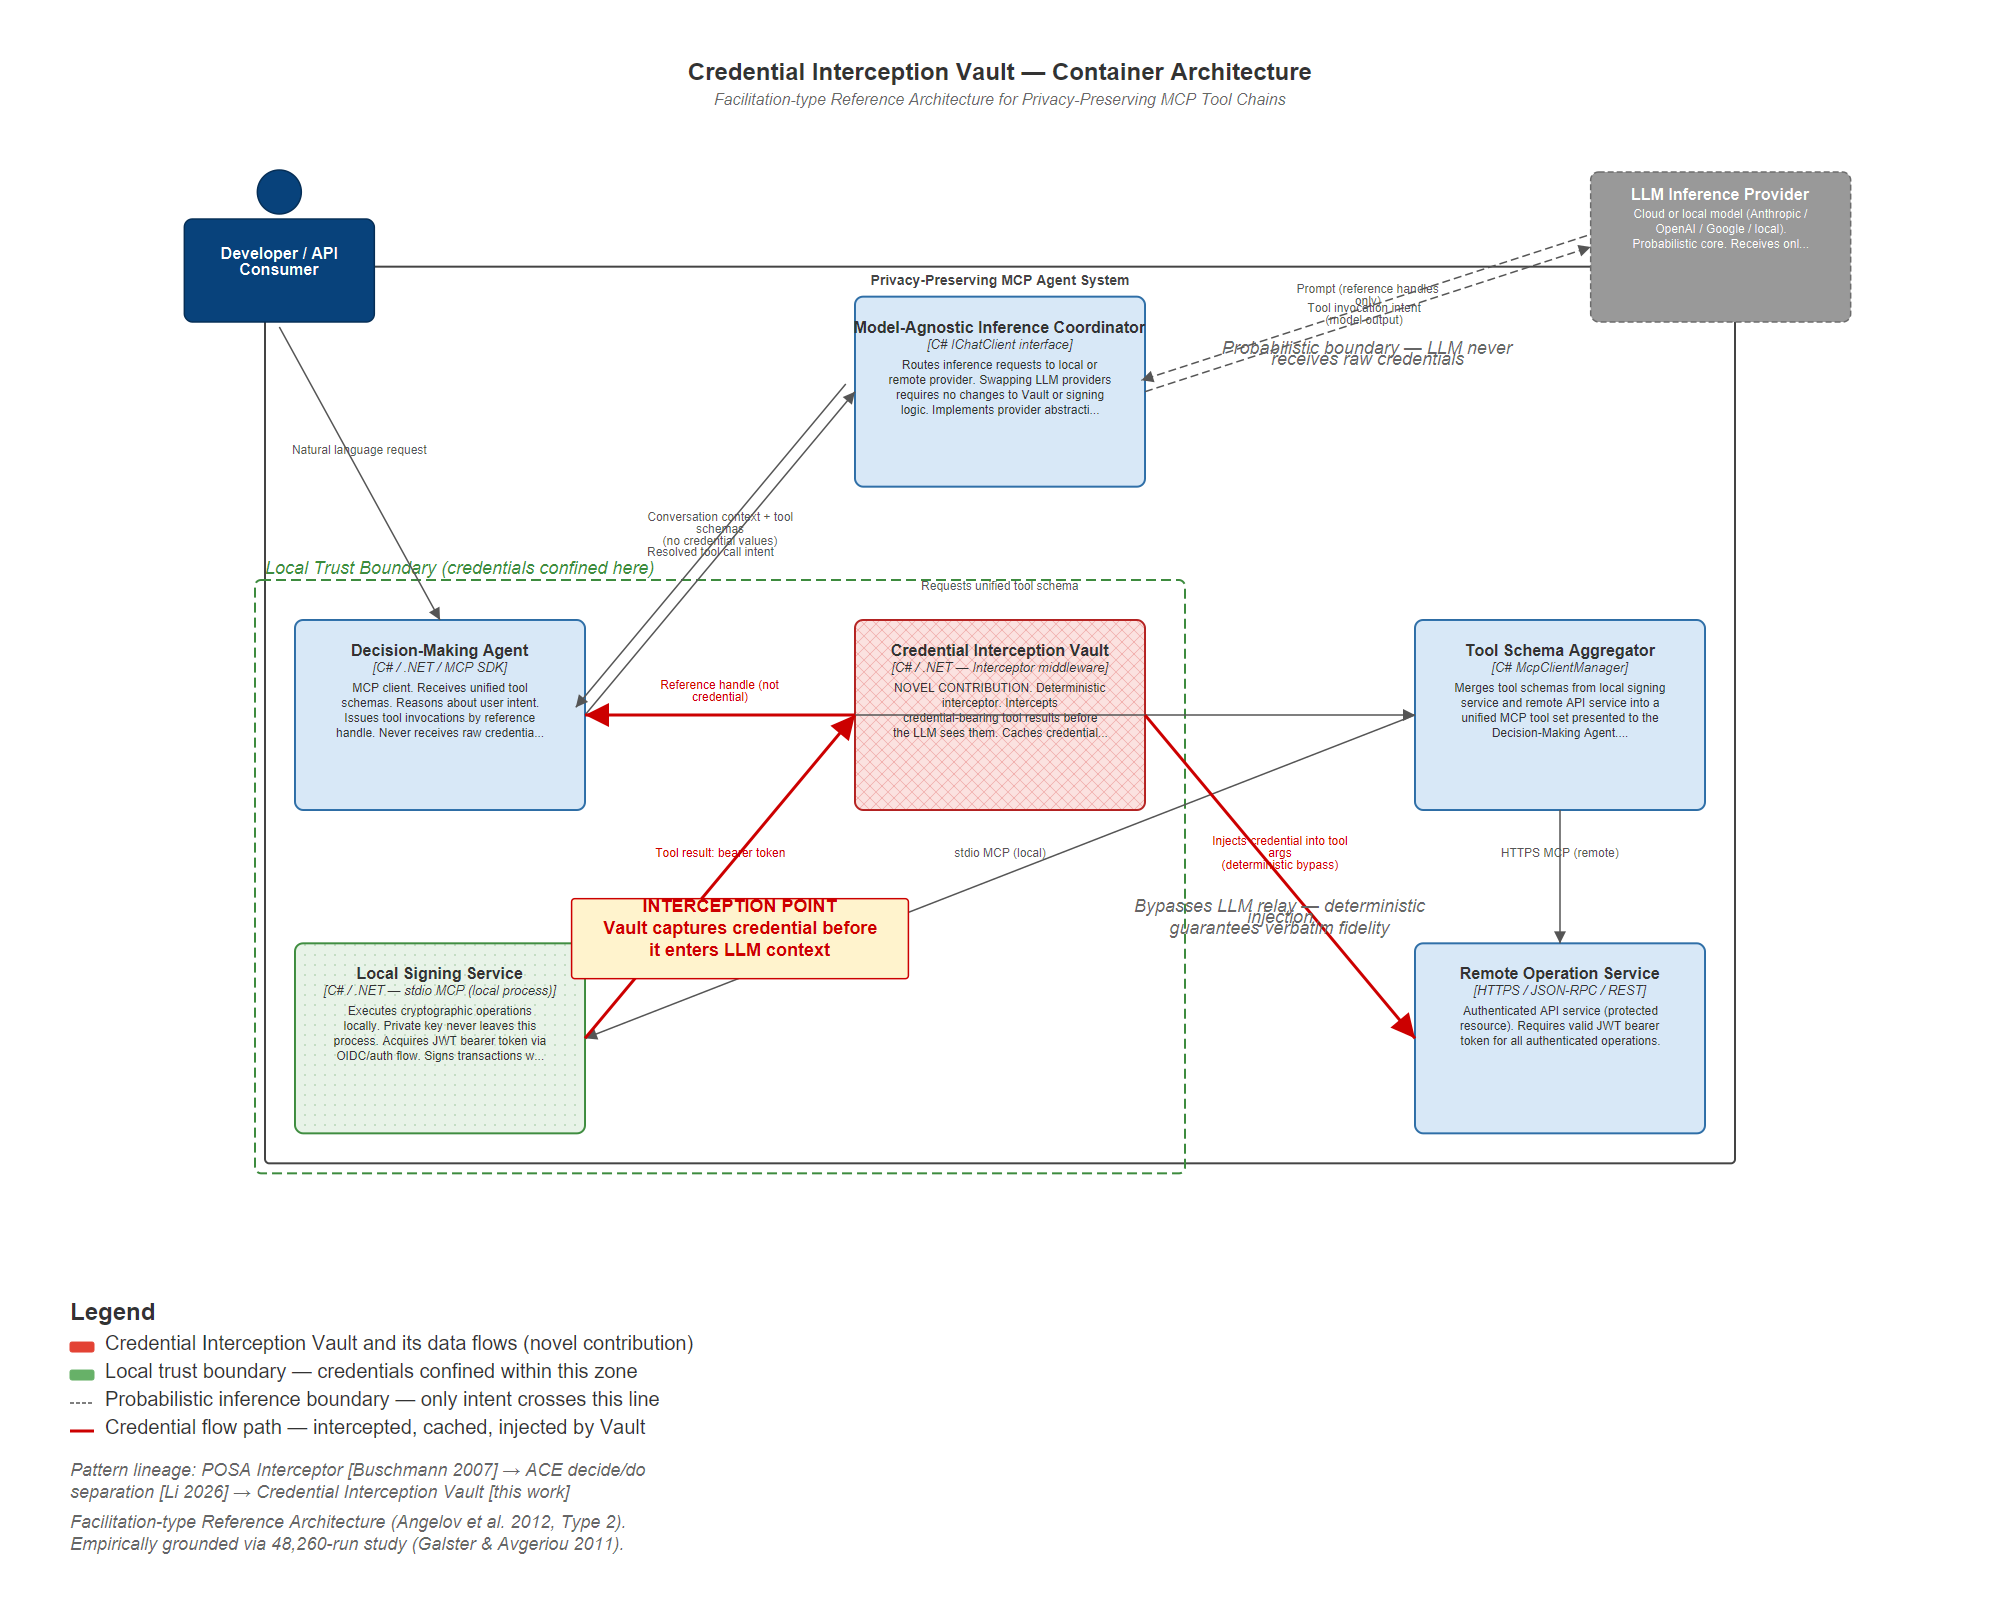
\includegraphics[width=0.99\textwidth]{figures/fig03_c4_container.png}
  \vspace{-4pt}\caption{Container-level view of the Credential Interception Vault
  reference architecture. The Vault (centre, red) is the invariant.
  Blue elements are variability points \texttt{[VP]}; grey elements are
  external actors/systems.
  Handle security model: see Section~\ref{sec:security}.}
  \label{fig:c4}
\end{figure*}

The five containers are the \emph{Decision-Making Agent} (MCP client, uses
only opaque handles); the \emph{Credential Interception Vault} (intercepts,
caches, and injects credentials); the optional \emph{Tool Schema Aggregator};
the \emph{Credential-Bearing Tool}~\texttt{[VP]}; and the \emph{Authenticated
Tool}~\texttt{[VP]}. External actors are the Service Consumer, LLM Inference
Provider (receives only handles, never raw credentials), and Protected
Resource~\texttt{[VP]}.

\subsection{Intercept-Cache-Inject Sequence}\label{sec:sequence}

Figure~\ref{fig:sequence} shows the runtime behaviour. The Vault
intercepts the credential-bearing tool result before it enters the LLM context
(\emph{intercept}), caches it under a fresh opaque handle (\emph{cache}), and
returns only the handle to the agent. When the agent issues a downstream tool
call, the Vault resolves the handle and injects the credential into the tool
arguments (\emph{inject}). No LLM re-encoding occurs between cache and injection.

\begin{figure*}[t]
  \centering
  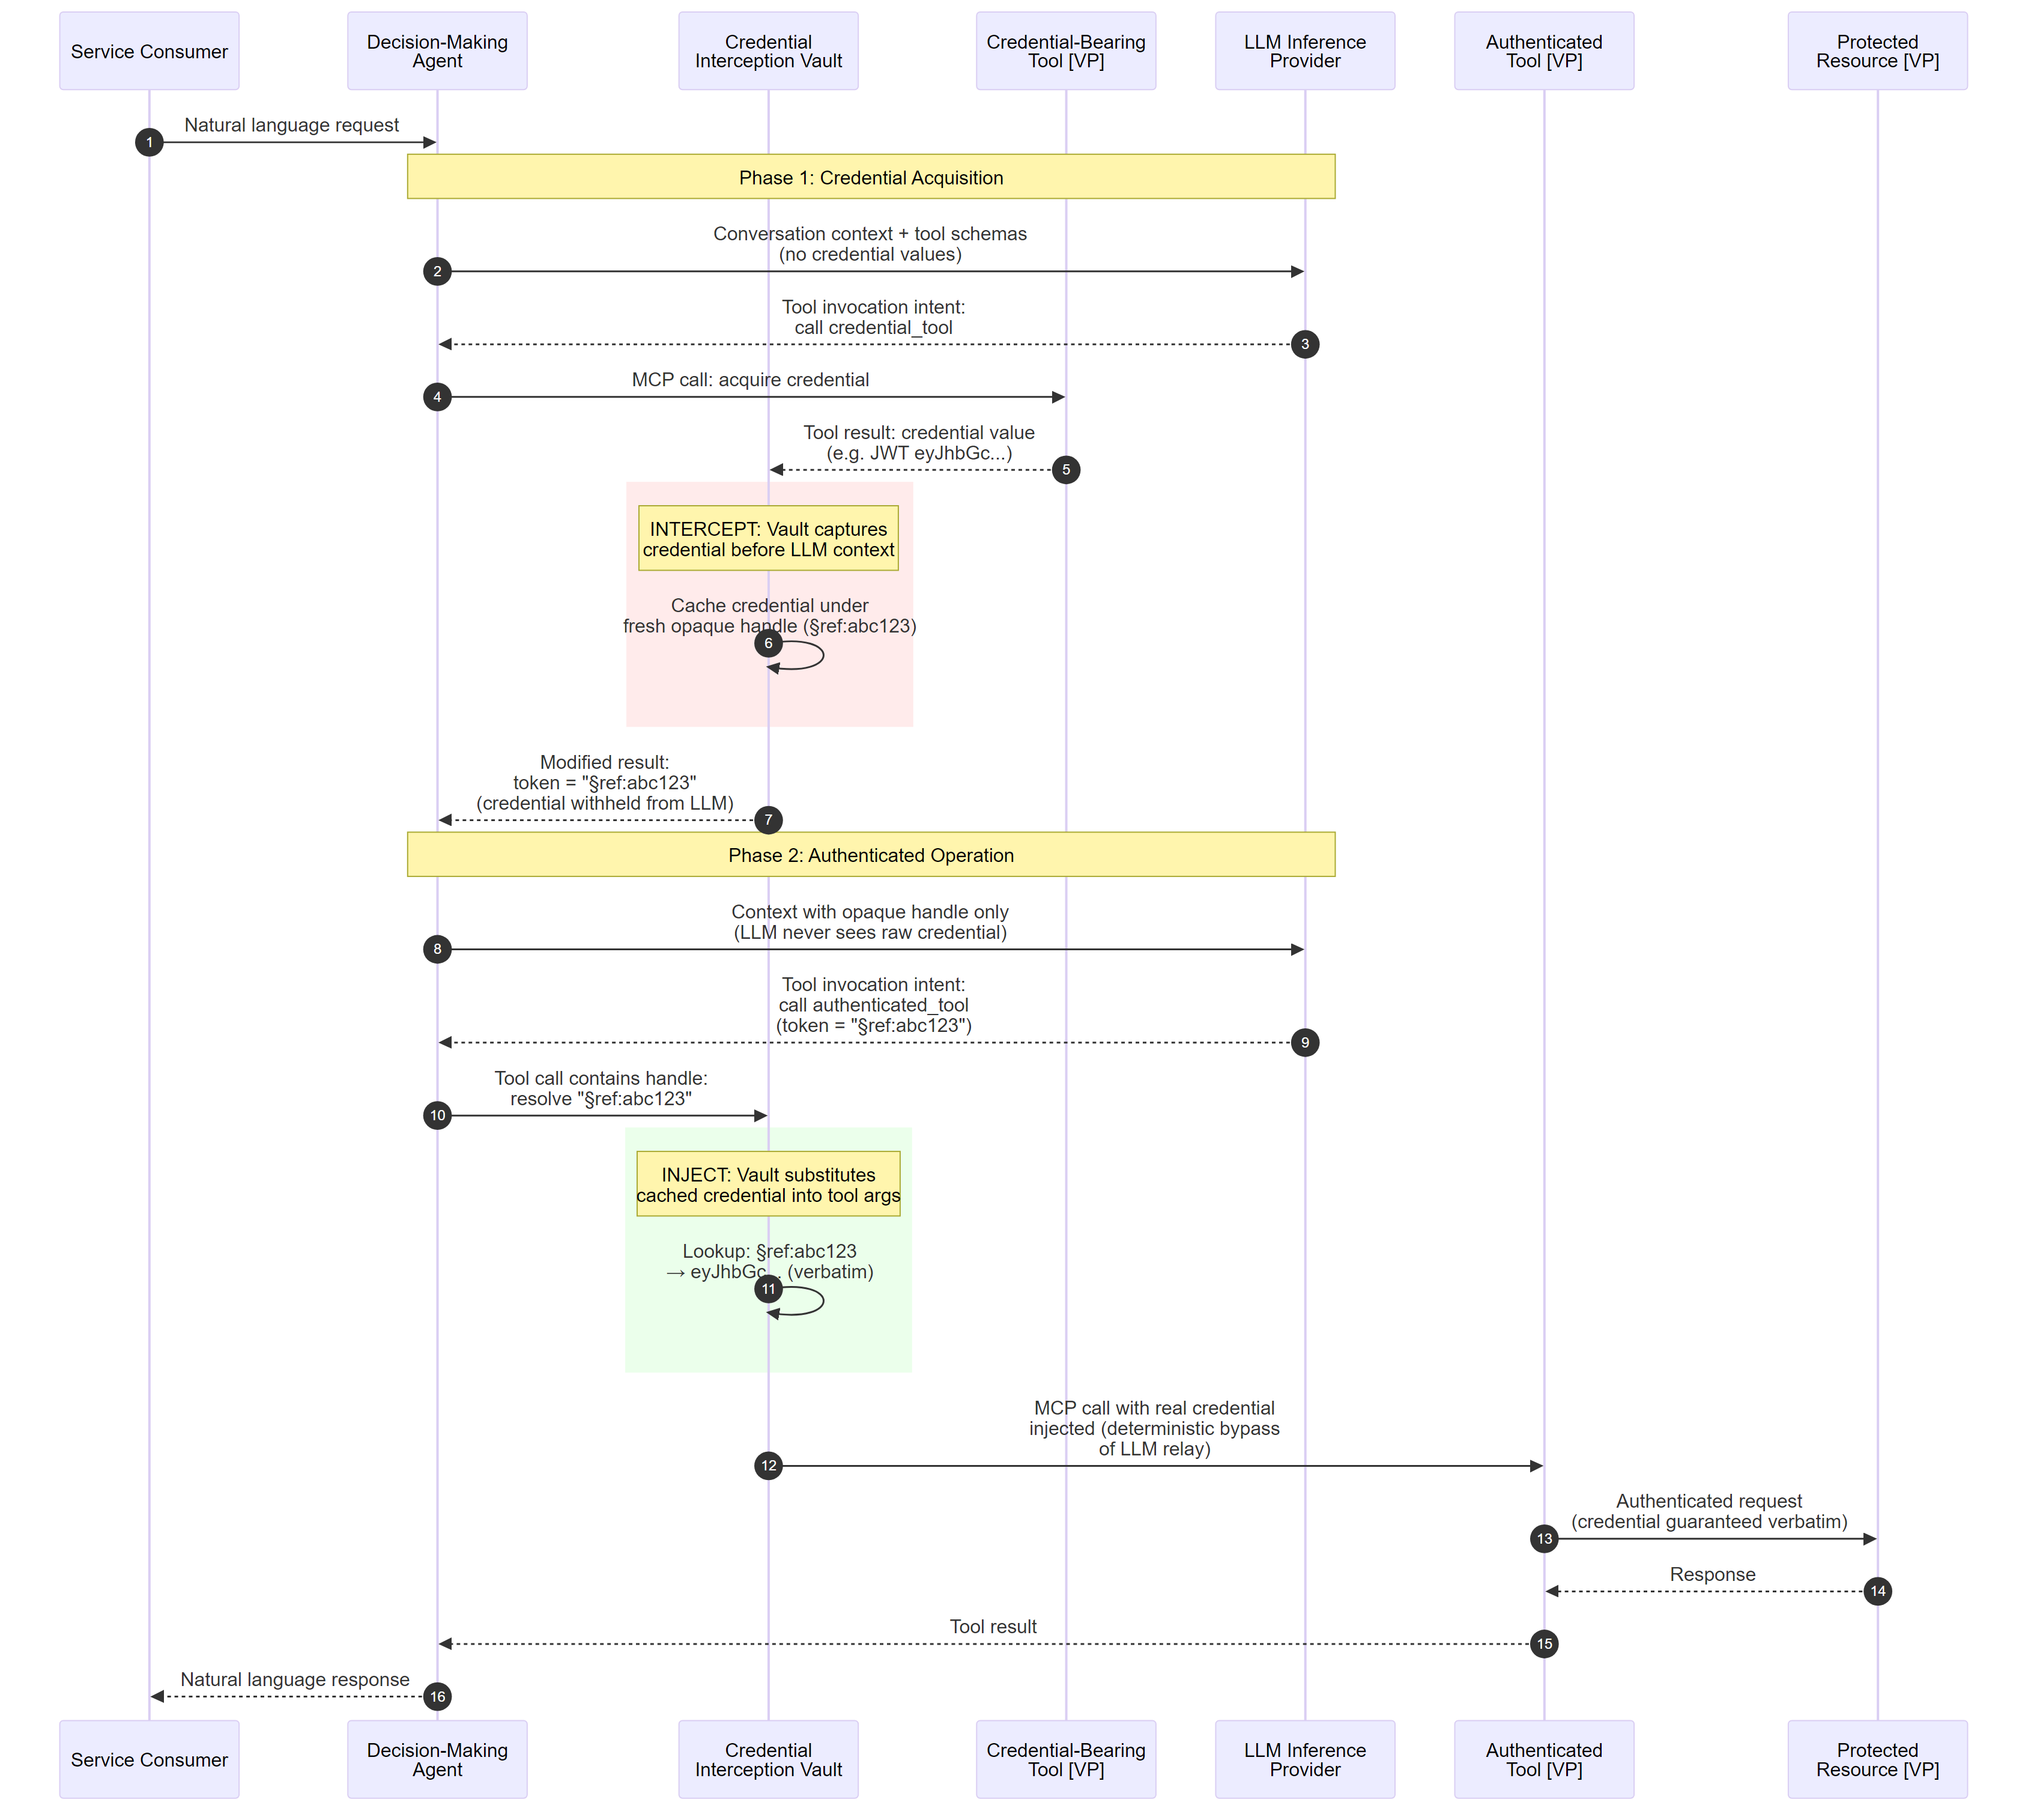
\includegraphics[width=0.75\textwidth]{figures/fig04_sequence.png}
  \vspace{-4pt}\caption{Intercept-cache-inject sequence for one credential relay cycle.
  The credential never enters the LLM context window. Steps 5--6 (red):
  intercept and cache. Steps 10--12 (green): resolve and inject.}
  \label{fig:sequence}
\end{figure*}

\subsection{Security and Privacy Properties}\label{sec:security}

\textbf{Confidentiality.} The credential never enters the LLM context window
and is never transmitted to the LLM inference provider. In deployments where
the provider is in a different jurisdiction and the credential constitutes
personal data (e.g., a user-specific bearer token), this property aligns with
GDPR Article~44 cross-border transfer restrictions~\cite{gdpr2016}.

\textbf{Integrity.} The cached credential is the authoritative copy.
Downstream injection is byte-for-byte identical to the cached original:
Levenshtein distance equals zero by construction, not by probabilistic
suppression. Cryptographic signature verification at the Protected Resource
succeeds with probability~1.0.

\textbf{Availability and concurrency.} The Vault runs in-process; network
partitions cannot interrupt injection. Handles are session-scoped UUIDs,
enabling stateless horizontal scaling.

\textbf{Handle security model.} Each handle is a cryptographically random
session-scoped UUID that carries no information about the credential's
content; an attacker who obtains a handle cannot derive the credential from
it. The handle lifecycle is: (i)~\emph{created} at intercept time and bound
to the current session; (ii)~\emph{resolved} exactly once per downstream
tool call; (iii)~\emph{expired} on session close or explicit invalidation,
after which the handle resolves to null and injection fails safe (the tool
call is rejected rather than forwarding a stale or empty credential).
Cross-session replay is rejected by construction: a handle UUID is absent
from a new session's store and therefore cannot be resolved. The trust
assumption is that the Vault runs within the local process trust boundary;
credentials and handles never cross that boundary to untrusted environments.

\textbf{Performance and interoperability.} The intercept-inject cycle adds one
in-memory lookup per relay event (sub-millisecond). The pattern is
protocol-agnostic and applies to any framework interposing tool-call results
before LLM context injection (LangChain, AutoGen, and similar runtimes);
each hop in a multi-hop chain intercepts independently.

% Section 6: Case Study
% Source: context/Case_Study_OpenOrderbook.md (all sections §CS1-§CS9)
% Source: context/Paper_Layout_Plan.md §6
%
% EM-DASH PROHIBITION: Do not use --- or \textemdash. Use colons or semicolons.

\section{Industrial Case Study}\label{sec:case_study}

This section addresses \RQ{5} using a mixed-method design: qualitative
triangulation across five evidence sources is augmented by the ecological
validity arm as an embedded controlled experiment (the no-Vault counterfactual).

\subsection{Case Context}\label{sec:case_context}

% ANON: All identifying details below are anonymised for double-anonymous review.
% Camera-ready version will name the company, product, and personnel with consent.

The case is a
\anon{production blockchain trading platform}{production OpenOrderbook/Upstream Exchange platform}
operated by
\anon{a Swiss-based fintech company}{Abbey Technologies GmbH}
serving approximately 13{,}000 registered users.
% ANON: company name, product name, exchange name
The platform provides fixed-return options trading in tokenised financial
instruments through an AI-native interface: an LLM orchestrator translates
trader instructions into on-chain operations via MCP tool chains. The
blockchain infrastructure is a private Proof-of-Authority (PoA) Ethereum-compatible
network with four active nodes.

Authentication uses RS256~\cite{rfc7518} JWTs~\cite{rfc7519} issued by Azure AD B2C at approximately
1{,}080 characters, placing the production tokens in the \emph{very long} tier
of our experimental design (Section~\ref{sec:objects}). A single character
corruption invalidates the RSA signature and produces an HTTP~403
rejection at the downstream API~\cite{rfc6750}. The LLM configuration supports multiple
providers (the controlled study includes Claude, GPT, and Gemini families);
a local privacy-preserving mode using Gemma~4~E4B (4B-parameter open-weight,
Ollama) is also supported for data-sovereignty deployments.

\textbf{Concrete instantiation.}
\texttt{[VP:~LLM]} = user-configurable model; \texttt{[VP:~Protected Resource]} = PoA
Ethereum RPC + REST trading API; \texttt{[VP:~Credential-Bearing Tool]} = RS256
signing service issuing Azure AD B2C JWTs.

\subsection{Evidence Sources}\label{sec:evidence}

Five independent evidence sources are triangulated. (1)~Production source code
and git commit history provide an objective timeline of mitigations.
(2)~Contemporaneous developer communications document the misdiagnosis phase
and the qualitative observation that prompting ``gave better results.''
(3)~A structured interview with
\anon{the company's CEO and infrastructure engineer}{Brian Collins and Pete Hall}
% ANON: personnel names
provides architectural context and co-author fact verification.
(4)~The ecological validity arm ($N\!=\!1{,}600$) serves a dual role: it
quantifies the production-specific \DFR{} for the main study, and it
constitutes the controlled counterfactual strand of this case study---the
\emph{no-Vault} condition instantiated on the actual production system via
an environment variable flag (\texttt{RESEARCH\_RAW\_MODE=true}), providing
a quantified baseline against which the post-Vault observation is interpreted. (5)~Commit-level pre/post evidence confirms zero
authentication failures after Vault deployment. No source contradicts another.

\subsection{Discovery Trajectory}\label{sec:trajectory}

JWT corruption was first observed on 2026-04-03 during UAT testing, eight days
after the MCP server was first built. The observable symptom was intermittent
\texttt{HTTP 403 Unauthorized} responses from the downstream REST API on
authenticated trading operations. The intermittent failure rate was
approximately 20\%, consistent with the very-long tier \DFR{} in the
controlled study.

\textbf{Misdiagnosis.}
The failure was attributed to infrastructure: signatures failed
\texttt{RSA.VerifyData()} against all six active JWKS keys. One key was 47 days
old, leading to the hypothesis that Azure AD was issuing tokens with a stale
private key; a Microsoft Support case was raised. The misdiagnosis was plausible:
a JWT corrupted by single-character substitution is cryptographically
indistinguishable from a token signed with an invalid key.

\textbf{Root cause identification.}
\anon{The lead developer}{Andrew Le Gear},
% ANON: personnel name
who had personally observed the corruption during testing, independently
formed the LLM relay hypothesis from knowledge of how LLMs handle opaque,
high-entropy strings. A diagnostic mechanism was added to the tool chain: the
\texttt{acquire\_bearer\_token} tool was modified to return a
\texttt{tokenFingerprint} (SHA256[:16] of the JWT), and a verification tool
was added to compute the fingerprint of the received bearer token. Comparing
fingerprints before and after LLM relay confirmed that the token was being
altered in transit.

\textbf{Prompting-first mitigation.}
The initial response followed a prompting-first trajectory: a 318-character
\texttt{CRITICAL} verbatim fidelity instruction was added to the
\texttt{bearerToken} parameter in the tool registry. The instruction explicitly
names the RSA signature consequence and the single-character precision
requirement.
The partial improvement confirmed the relay hypothesis but did not solve the
problem. This is precisely the intervention evaluated in the ecological
validity arm (Section~\ref{sec:eco_results}): the same 318-character
instruction, the same production JWT schema, producing 19.9\% residual \DFR{}.

\textbf{Architectural solution.}
On 2026-04-13 (commit \texttt{5df1b265a}),
\anon{the lead developer}{Le Gear}
% ANON: personnel name
deployed the Vault implementation, with the commit comment: \emph{``Bearer token
vault: bypass the LLM to prevent token corruption. The LLM hallucinates data
into JWT tokens (expanding claims, appending fake responses). We intercept the
token from acquire\_bearer\_token results and inject it directly.''}
This comment identifies two failure modes observed in production:
(1)~semantic expansion, where the LLM hallucinated additional JSON claims
into the JWT payload; and (2)~content fabrication, where the LLM appended
fabricated tool-response content after the JWT. Both are consistent with the
failure taxonomy in Table~\ref{tab:taxonomy}.

The commit message uses no architectural pattern vocabulary; the solution was
derived from first principles under production pressure. Pattern identification
and naming were applied retrospectively, confirming the RA as a naturally
emerging solution that this paper names, formalises, and validates.

\subsection{Reactive Mitigations as Defence-in-Depth}\label{sec:reactive}

Before the Vault was implemented, and retained alongside it as defence-in-depth,
two reactive mitigation layers were added to the MCP handler. The first,
\texttt{SanitizeBearerToken()}, handles structural failures: it extracts the
\texttt{accessToken} field when the LLM passes the full JSON response object
(case~1), strips non-Base64url characters appended after the signature
(case~2), and removes \texttt{Bearer} prefix confusion (case~3). The second,
\texttt{JwtValidator.ValidateAndRepairAsync()}, implements single-character
brute-force repair of RS256 signatures: for each character position in the
signature segment, it substitutes all 64 Base64url characters and tests
\texttt{RSA.VerifyData()} against the JWKS keys. This repairs Levenshtein-1
corruption in the signature segment but cannot repair multi-character corruption
or payload-level semantic substitution.

Table~\ref{tab:coverage} maps these layers against the failure taxonomy. The
reactive mitigations cover format errors and low-Levenshtein signature
corruption but cannot detect semantic substitution (\texttt{sem\_sub}), where
the corrupted token is well-formed and plausible-length. The Vault is the only
mechanism with complete coverage: it bypasses the failure mode entirely by
removing the credential from the LLM's inference path.

\begin{table}[t]
\centering
\footnotesize
\vspace{-4pt}\caption{Defence-in-depth coverage matrix. Reactive mitigations cover a subset
of failure modes; the Vault covers all by bypassing LLM relay.}
\label{tab:coverage}
\begin{tabular}{@{}lccc@{}}
\toprule
\textbf{Failure mode} & \textbf{Sanitize} & \textbf{Validator} & \textbf{Vault} \\
\midrule
JSON object relay        & \checkmark & Partial & \checkmark \\
Trailing fabrication     & \checkmark & Partial & \checkmark \\
Bearer prefix confusion  & \checkmark & Partial & \checkmark \\
Char-level substitution  & $\times$   & \checkmark & \checkmark \\
Multi-char corruption    & $\times$   & $\times$   & \checkmark \\
Abstention / refusal     & $\times$   & $\times$   & \checkmark \\
\bottomrule
\end{tabular}
\end{table}

\subsection{Ecological Validity}\label{sec:eco_results}

The eco arm ($N\!=\!1{,}600$; 16 models $\times$ 100 iterations) is the
controlled counterfactual for this case study. It used the exact production JWT
schema (1{,}080-character RS256 Azure AD B2C token) and the verbatim
318-character \texttt{BearerTokenParam} instruction from the production
codebase, executed through the production software with Vault protection
deliberately disabled. An environment variable flag (\texttt{RESEARCH\_RAW\_MODE=true}, commit
\texttt{2396d5273}, 2026-07-07) bypasses both \texttt{SanitizeBearerToken()}
and \texttt{JwtValidator}, forwarding the raw LLM output verbatim to the
downstream API. The production binary is identical in both modes; only the
runtime environment variable differs, ensuring the treatment and control
conditions share the same code path and differ solely in the presence or
absence of Vault interception. This design was necessary because the
production mitigations are effective enough to mask the underlying failure:
without deliberately disabling them, the raw \DFR{} is not observable.

The eco arm \DFR{} was 19.9\%, a $+1.9$ percentage point difference from the
main study ($p\!=\!0.16$, Wilcoxon; not
significant). The Spearman rank correlation between eco arm and main experiment
model rankings was $\rho\!=\!0.740$ ($p\!=\!0.001$), confirming that model
rankings transfer to production conditions.

\subsection{Post-Vault Deployment}\label{sec:post_vault}

Zero JWT authentication failures have been recorded over the 88-day observation
window from Vault deployment (2026-04-13) through 2026-07-10. Azure Monitor
metrics record 4{,}774 MCP tool invocations during this window; at the eco
arm's 19.9\% \DFR{}, approximately 950 would have failed without Vault
protection. The eco arm (Section~\ref{sec:eco_results}) provides the quantified
counterfactual on the same production system.
The post-Vault zero-failure observation is interpreted against that baseline,
not in isolation. This is a structural result, not a statistical one: the Vault
eliminates the failure mode by removing the credential from the LLM's inference
path. The expected post-Vault \DFR{} is not ``lower than 18.0\%'' but exactly
zero by construction for the byte-relay property: the byte sequence injected
into each outbound request is identical to the credential stored in the Vault.
This guarantee does not extend to credential theft, token expiry, revocation,
or replay attacks, which require independent controls.

% Section 7: Discussion
% Source: context/Discussion_and_Conclusions.md §D2-D8
% Source: context/ICSA_RA_Literature_Review.md §12
%
% EM-DASH PROHIBITION: Do not use --- or \textemdash. Use colons or semicolons.

\section{Discussion}\label{sec:discussion}

The empirical findings and case study evidence converge on a single conclusion:
LLM credential relay corruption is a systematic failure mode that prompt
engineering did not eliminate in any condition tested, motivating an architectural
response. We discuss six implications.

\textbf{Prompt engineering as insufficient mitigation.}
The production system deployed the most explicit bearerToken instruction
achievable within the MCP tool schema (318 characters naming the RSA mechanism,
the 403 consequence, and single-character precision). It produced 19.9\%
\DFR{} ($p\!=\!0.16$; a null result, not a positive equivalence claim). BPE tokenisation
boundaries \emph{appear} to operate below the instruction-following layer; no
instruction eliminated corruption in any of the 16 models tested. In the conditions
evaluated, prompt improvement was bounded at $\sim$5~pp (L1-to-L3) with no approach toward zero. We present
this as an \emph{observed practical insufficiency}: the most aggressive prompting
strategy available under MCP schema constraints did not reduce \DFR{} to an
acceptable level for cryptographic relay. Formal equivalence testing (TOST with a pre-specified margin)
remains future work; the current finding is sufficient to motivate an
architectural bypass.

\textbf{Mitigation vs.\ bypass: a category difference.}
The Vault achieves zero \DFR{} by construction for the byte-relay property
(a design argument, not an additional empirical measurement): removing the
credential from inference makes byte-level corruption architecturally
impossible. This guarantee is scoped to relay fidelity; it does not address
credential theft at rest, token expiry, revocation, or replay attacks;
those remain the responsibility of the surrounding identity infrastructure. Prompt-based mitigation asks how to
make the LLM relay more reliably; \DFR{} remains above zero. These are
solutions to different problems. Bypass is appropriate when correctness is
required (RSA verification is binary), when the failure is
unrecoverable (HTTP~403 with no retry), and when credentials are sensitive personal data~\cite{gdpr2016}.

\textbf{When to apply the Vault.}
Apply when: (i)~credential length exceeds $\sim$200~chars;
(ii)~a cryptographic signature is present; or (iii)~a relay error is unrecoverable.
Prompt mitigation may suffice in retry-tolerant contexts below that threshold.

\textbf{Organic convergence validates the RA.}
The production Vault was implemented independently without reference to
this research (Section~\ref{sec:trajectory}), confirming the RA as
naturally emergent and transferable without requiring rediscovery.

\textbf{Credential lengths are increasing; the risk may worsen.}
Gibberish bias intensifies with larger vocabularies~\cite{chen2026gibberish}.
NIST key sizes~\cite{barker2020nistkeys} and post-quantum
algorithms~\cite{nist2024pqc} (CRYSTALS-Dilithium: 2{,}420~bytes; SPHINCS+:
7{,}856~bytes) would push tokens deeper into the high-\DFR{} tier, making 17.3\% a
conservative lower bound (this projection requires empirical validation). The
Vault addresses this trajectory without modification.

\textbf{Broader implications for agentic AI systems.}
As LLM-based agent systems proliferate~\cite{wang2024survey}, any opaque
high-entropy string (API keys, hash digests, certificate fragments) may share
the same distribution-shift vulnerability. JWT relay is the validated case;
extension to other credential classes is a hypothesis requiring independent
empirical confirmation. The eco arm
($\rho\!=\!0.740$) provides a reusable calibration instrument for
deployment-specific risk.

% Section 8: Threats to Validity
% Source: context/Discussion_and_Conclusions.md §D9
%
% EM-DASH PROHIBITION: Do not use --- or \textemdash. Use colons or semicolons.

\section{Threats to Validity}\label{sec:threats}

\textbf{Construct validity.}
The binary \DFR{} metric does not capture corruption severity, but RSA
verification is itself binary (any distance $>0$ is fatal), making the metric
appropriate. Synthetic JWTs may under-represent real-world complexity; the eco
arm mitigates this by running with the exact production schema
($\sim$1{,}080~chars, RS256 Azure AD B2C) and obtaining
\DFR{}~=~19.9\%, statistically indistinguishable from the synthetic result.

\textbf{Internal validity.}
Experiments used direct provider API calls; identical corruption patterns
across six independent provider SDKs make a middleware artifact implausible.
All models were accessed under pinned version identifiers during a fixed
collection window of 3--7~July~2026; any residual within-study drift is
accounted for by the GEE clustering structure. Provider back-end updates
between study start and end could introduce uncontrolled variance; the fixed
collection window and version pinning limit but do not eliminate this risk.
The tokenisation hypothesis is the most parsimonious explanation for the
observed length-gating pattern; alternative mechanisms (tool-call
serialisation artefacts, provider SDK transforms, safety-layer rewrites)
have not been experimentally ruled out. Causal attribution is out of scope
for this study, whose primary contribution is demonstrating that the problem
exists at meaningful scale and that an architectural bypass eliminates it.

\textbf{External validity.}
The 16 models cover eight tiers and six providers but do not represent
the full model landscape; new models may exhibit different failure profiles.
The eco arm's $\rho\!=\!0.740$ rank correlation supports transfer to at least one
production deployment; generalisation to other credential types or schemas
requires future work (Section~\ref{sec:discussion}).
Per-model eco breakdowns are in the replication package.

\textbf{Conclusion validity.}
Multiple comparisons across 16 models inflate Type~I error; all pairwise
comparisons are corrected by Benjamini-Hochberg at FDR~=~0.05. The primary
inference (\DFR{} $> 0$\% across all models) is a single test with effectively
unlimited power at $N\!=\!50{,}400$. The analysis plan was pre-registered
before data collection to reduce observer bias.

% Section 9: Conclusion
% Source: context/Discussion_and_Conclusions.md §D11
%
% EM-DASH PROHIBITION: Do not use --- or \textemdash. Use colons or semicolons.

\section{Conclusion}\label{sec:conclusion}

LLM credential relay corruption is not an edge case. Across 50{,}400 main-arm runs
with 16 frontier models, the JWT defect rate was 18.0\% (range 0.5--99.8\%;
12.5\% excluding Mistral Large~3), with no model achieving zero corruption.
The eco arm confirmed a residual \DFR{} of 19.9\% under the most explicit
production instruction ($p\!=\!0.16$). The Credential Interception Vault
eliminates the failure by removing the credential from inference; zero
authentication failures have been recorded since deployment.

The seven contributions (Section~\ref{sec:introduction}) span empirical
characterisation (\Contrib{1}--\Contrib{4}), the Credential Interception Vault
RA (\Contrib{5}), industrial validation (\Contrib{6}), and an open replication
package (\Contrib{7}).

Credential lengths are increasing~\cite{barker2020nistkeys,nist2024pqc},
deepening the corruption risk. The Vault provides a principled, model-agnostic,
and empirically validated answer. For practitioners building MCP tool chains:
do not relay credentials exceeding $\sim$200 characters through LLM inference;
intercept them deterministically at the middleware layer.


% ─── Acknowledgment (anonymous for submission) ───────────────────────
% ANON: Uncomment for camera-ready version
\vspace{-4pt}\section*{Acknowledgment}
\vspace{-5pt}
{\small\anon{This research was conducted within [anonymised], the [anonymised]
Research Centre for Software, funded by [anonymised] under grant [anonymised]
in conjunction with [anonymised] under statement of work [anonymised].}{This
research was conducted within Lero, the Science Foundation Ireland Research
Centre for Software, funded by Research Ireland (grant 13/RC/2094) (SOWP2-TP0063).}}

\vspace{-6pt}\section*{Ethics Statement}
\vspace{-5pt}
{\small\anon{Ethical approval was granted by [institution withheld] under expedited
review (reference withheld). The industry partner provided written consent for
the case study.}{Ethical approval was granted by the University of Limerick
Research Ethics Committee (ref.\ 2026-07-XX). Abbey Technologies GmbH provided
written consent for the case study and for the company to be named.}}

\vspace{-6pt}\section*{AI Disclosure}
\vspace{-5pt}
{\small Microsoft Copilot assisted with spelling and grammar; all intellectual
content is the authors' own.}

\vspace{-10pt}\section*{Data Availability}
\vspace{-5pt}
{\small Replication package:
\anon{\url{https://anonymous.4open.science/r/jwt-mcp-replication-FF50/}}{\url{https://github.com/andylegear/jwt-mcp-replication}}.
% ANON: Replace anonymous.4open.science URL with real GitHub URL for camera-ready
Experiment database (${\approx}161$\,MB, 52{,}000 runs):
\url{https://osf.io/5zd42/} (SHA-256: \texttt{ac1de7ac\ldots fdc5c0e}).}

% ─── References ──────────────────────────────────────────────────────────────
% \balance  % disabled: let columns be unequal so boilerplate stays on p10
\bibliographystyle{IEEEtran}
\bibliography{references}

\end{document}
